\chapter{Pengenalan Machine Learning: Supervised Learning}

\section{Peran Machine Learning dalam Era Big Data}

Perkembangan teknologi dan meningkatnya kemampuan organisasi dalam mengumpulkan serta menyimpan data dalam jumlah besar telah mendorong lahirnya era Big Data. Karakteristik Big Data yang dikenal dengan 5V — volume, velocity, variety, veracity, dan value — menggambarkan kompleksitas sekaligus potensi yang dapat dimanfaatkan untuk keunggulan kompetitif \cite{laney2001,gandomi2015,nist2015}.

Dalam konteks ini, \textbf{Machine Learning (ML)} menjadi komponen krusial dalam \textit{Big Data Value Chain}, khususnya pada tahapan analisis dan ekstraksi wawasan setelah proses integrasi dan penyimpanan data. ML memungkinkan organisasi untuk berpindah dari analisis deskriptif ke arah analisis prediktif dan preskriptif yang jauh lebih bernilai dalam pengambilan keputusan \cite{chen2012,wamba2017}.

Berbagai sektor bisnis telah menerapkan ML untuk berbagai keperluan, antara lain:
- Prediksi churn pelanggan di industri telekomunikasi dan ritel,
- Deteksi penipuan dalam sektor keuangan,
- Prediksi permintaan di rantai pasok,
- Rekomendasi produk di e-commerce \cite{mcafee2012,mariani2021,georgescu2020}.

Secara strategis, ML memperluas cakupan manfaat Big Data dari sekadar "pengetahuan tentang masa lalu" menjadi "pengetahuan tentang masa depan" melalui kemampuan prediksi berbasis pola data historis. Hal ini memungkinkan organisasi untuk membuat keputusan yang lebih cepat, tepat, dan terukur \cite{jeble2018,oecd2015,assuncao2015}.

Dalam konteks Big Data for Business, pemahaman dasar tentang ML, khususnya supervised learning, menjadi bekal penting bagi pengambil keputusan non-teknis agar dapat berkolaborasi secara efektif dengan tim data dan memanfaatkan hasil model secara optimal untuk kepentingan strategis organisasi \cite{provost2013data,fernandez2020,davenport2018}.



\section{Pengantar Machine Learning}

\textbf{Machine Learning (ML)} merupakan cabang dari kecerdasan buatan yang memungkinkan komputer belajar dari data tanpa perlu diprogram secara eksplisit untuk setiap aturan atau kondisi. Secara intuitif, ML bekerja dengan cara mengenali pola dalam data historis dan menggunakan pola tersebut untuk membuat prediksi atau keputusan terhadap data baru \cite{kelleher2015fundamentals}.

Dalam konteks analisis data bisnis, pendekatan konvensional (berbasis aturan) biasanya mengandalkan logika "jika–maka" yang ditentukan oleh pakar atau pengembang sistem. Sebagai contoh, dalam sistem deteksi penipuan berbasis aturan, programmer akan menetapkan aturan seperti: \textit{jika transaksi lebih dari 100 juta dan dilakukan di luar negeri, maka flag sebagai penipuan}. Meskipun efektif untuk skenario yang diketahui sebelumnya, pendekatan ini memiliki keterbatasan dalam skala besar, variasi tinggi, serta dinamika data yang terus berubah.

Sebaliknya, pendekatan Machine Learning memungkinkan sistem untuk secara otomatis membangun model dari data yang tersedia. Dengan menyediakan data historis yang telah diberi label (misalnya: transaksi yang diketahui sebagai penipuan atau bukan), algoritma ML akan mempelajari pola dan relasi antar variabel untuk kemudian digunakan pada data baru. Hal ini sangat berguna dalam menghadapi kompleksitas data bisnis modern yang tidak dapat ditangani hanya dengan aturan eksplisit.

ML juga bersifat adaptif. Model dapat diperbarui seiring waktu dengan data terbaru, sehingga tetap relevan dalam lingkungan bisnis yang dinamis. Contohnya, sistem rekomendasi produk pada platform e-commerce dapat belajar dari riwayat pembelian dan perilaku pengguna, kemudian menyesuaikan rekomendasi secara personalisasi.

Oleh karena itu, pemahaman terhadap prinsip dasar Machine Learning menjadi semakin penting bagi para pengambil keputusan di bidang bisnis dan manajemen, terutama dalam era Big Data yang menuntut kecepatan, akurasi, dan skalabilitas dalam pengambilan keputusan berbasis data.


\section{Tipe-Tipe Learning pada Machine Learning }

Machine Learning (ML) dapat diklasifikasikan ke dalam tiga tipe utama berdasarkan cara model belajar dari data, yaitu: \textbf{supervised learning}, \textbf{unsupervised learning}, dan \textbf{reinforcement learning} \cite{provost2013data}.

\textbf{1. Supervised Learning}  
Supervised learning adalah tipe machine learning di mana model belajar dari data yang sudah diberi label, artinya setiap data input (fitur) disertai dengan output yang benar (label). Tujuannya adalah agar model dapat mempelajari hubungan antara input dan output tersebut, sehingga dapat memprediksi output baru secara akurat.  
Contoh umum dalam bisnis meliputi:
- \textit{Prediksi churn pelanggan}: menggunakan riwayat transaksi dan interaksi pelanggan untuk memprediksi apakah pelanggan akan berhenti berlangganan.
- \textit{Estimasi penjualan}: memprediksi jumlah penjualan produk berdasarkan musim, lokasi, dan tren sebelumnya.
- \textit{Kredit scoring}: memprediksi risiko gagal bayar berdasarkan histori kredit dan data demografis.

Supervised learning merupakan pendekatan yang paling umum digunakan dalam aplikasi bisnis karena tersedia banyak data historis yang telah diberi label, dan hasil prediksinya mudah diinterpretasikan oleh pengambil keputusan \cite{chen2012,davenport2018}.

\textbf{2. Unsupervised Learning}  
Unsupervised learning digunakan ketika data tidak memiliki label. Tujuannya adalah menemukan struktur atau pola tersembunyi di dalam data.  
Contoh penerapannya dalam bisnis:
- \textit{Segmentasi pelanggan}: mengelompokkan pelanggan ke dalam segmen berdasarkan perilaku, preferensi, atau profil.
- \textit{Deteksi anomali}: menemukan transaksi mencurigakan tanpa diberi label penipuan secara eksplisit.

Teknik umum dalam unsupervised learning termasuk \textit{clustering} (misalnya k-means) dan \textit{dimensionality reduction} (misalnya PCA).

\textbf{3. Reinforcement Learning}  
Reinforcement learning adalah pendekatan di mana agen belajar dengan berinteraksi dengan lingkungan dan menerima umpan balik dalam bentuk \textit{reward} atau \textit{penalty}. Tujuan agen adalah memaksimalkan reward jangka panjang.  
Meskipun lebih banyak digunakan dalam bidang robotika dan game, beberapa aplikasi bisnis mulai muncul, seperti:
- \textit{Dynamic pricing}: menyesuaikan harga produk secara adaptif berdasarkan permintaan pasar.
- \textit{Optimasi penempatan iklan}: menentukan urutan atau tampilan iklan untuk memaksimalkan klik atau konversi.

\textbf{Fokus pada Supervised Learning dalam Bisnis}  
Dalam konteks Big Data for Business, supervised learning menjadi titik awal yang ideal karena:
- Data historis bisnis umumnya telah memiliki label (misalnya status transaksi, churn, pembelian),
- Hasil model dapat digunakan untuk prediksi yang langsung mendukung keputusan operasional dan strategis,
- Model relatif mudah dievaluasi menggunakan metrik seperti akurasi, precision, dan recall.

Dengan demikian, pemahaman tentang supervised learning sangat penting bagi praktisi bisnis non-teknis untuk memahami cara kerja model prediksi dan bagaimana menggunakannya secara bertanggung jawab dalam pengambilan keputusan berbasis data \cite{provost2013data}.


\section{Konsep Dasar Supervised Learning}

Supervised learning adalah pendekatan machine learning yang bekerja dengan cara mempelajari hubungan antara \textbf{fitur (X)} sebagai input dan \textbf{label (Y)} sebagai output. Dalam konteks bisnis, fitur adalah data atau atribut yang menggambarkan karakteristik entitas yang diamati, sedangkan label adalah hasil atau status akhir yang ingin diprediksi \cite{provost2013data}.

Sebagai contoh, jika kita ingin memprediksi apakah seorang pelanggan akan berhenti berlangganan layanan (churn), maka:
\begin{itemize}
	\item Fitur (\textit{X}): jumlah panggilan layanan pelanggan, total penggunaan dalam sebulan terakhir, status pembayaran, durasi berlangganan.
	\item Label (\textit{Y}): \texttt{1} jika pelanggan berhenti, \texttt{0} jika tetap menggunakan layanan.
\end{itemize}

Supervised learning terbagi menjadi dua jenis utama berdasarkan tipe label yang diprediksi:

\subsection*{1. Klasifikasi (Classification)}
Klasifikasi digunakan ketika label (\textit{Y}) berupa kategori atau kelas diskrit. Tujuannya adalah menentukan kelas mana yang sesuai untuk sebuah data baru.  
Contoh aplikasi bisnis:
\begin{itemize}
	\item \textbf{Prediksi churn pelanggan}: apakah pelanggan akan berhenti atau tetap berlangganan (\texttt{Yes} / \texttt{No}).
	\item \textbf{Deteksi penipuan transaksi}: apakah transaksi termasuk normal atau fraud.
	\item \textbf{Klasifikasi kelayakan kredit}: apakah pemohon tergolong berisiko tinggi atau rendah.
\end{itemize}
Model yang umum digunakan untuk klasifikasi antara lain: Decision Tree, Logistic Regression, Random Forest, dan Support Vector Machine.

\subsection*{2. Regresi (Regression)}
Regresi digunakan ketika label (\textit{Y}) berbentuk nilai kontinu. Tujuannya adalah memprediksi nilai numerik berdasarkan fitur input.  
Contoh aplikasi bisnis:
\begin{itemize}
	\item \textbf{Estimasi penjualan bulan depan}: berdasarkan tren historis, musim, kampanye promosi, dan lokasi.
	\item \textbf{Prediksi pendapatan pelanggan}: mengestimasi lifetime value pelanggan berdasarkan perilaku pembelian.
	\item \textbf{Forecasting permintaan produk}: memprediksi permintaan harian atau mingguan berdasarkan variabel pasar.
\end{itemize}
Algoritma regresi yang umum digunakan meliputi: Linear Regression, Ridge/Lasso Regression, dan Gradient Boosting Regressor.

\subsection*{Mengapa Penting dalam Bisnis?}
Klasifikasi dan regresi merupakan dua jenis prediksi yang sangat sering digunakan dalam pengambilan keputusan strategis dan operasional berbasis data. Keduanya memungkinkan organisasi untuk merespons perubahan kondisi secara proaktif, mengurangi risiko, dan meningkatkan efisiensi \cite{chen2012}.

Dengan memahami konsep fitur dan label serta perbedaan antara klasifikasi dan regresi, pengambil keputusan non-teknis akan lebih mudah membaca hasil model, menilai implikasinya, dan mengintegrasikan ke dalam proses bisnis yang ada \cite{provost2013data}.


\section{Algoritma Populer untuk Supervised Learning}

Berbagai algoritma telah dikembangkan untuk supervised learning, masing-masing dengan kelebihan dan konteks penggunaan yang berbeda. Bagian ini akan menjelaskan empat algoritma yang paling sering digunakan dalam dunia bisnis, secara intuitif dan tanpa rumus.

\subsection*{1. Linear Regression}

\textbf{Linear Regression} adalah algoritma prediktif yang digunakan untuk memperkirakan nilai numerik (regresi), misalnya penjualan, pendapatan, atau permintaan produk.  
Cara kerjanya adalah mencari garis lurus terbaik yang menggambarkan hubungan antara fitur (misalnya jumlah iklan yang ditayangkan) dan label (misalnya jumlah penjualan).  
Contoh: Jika perusahaan ingin mengetahui bagaimana jumlah promosi digital memengaruhi total penjualan, linear regression dapat memberikan estimasi kuantitatif atas dampak tersebut.

\begin{figure}[h]
	\centering
	\begin{tikzpicture}[scale=1]
		
		% Axis
		\draw[->] (0,0) -- (6.5,0) node[below right] {Jumlah Promosi};
		\draw[->] (0,0) -- (0,5) node[above left] {Penjualan};
		
		% Sample data points
		\filldraw[blue] (0.5,1.2) circle (2pt);
		\filldraw[blue] (1.5,1.6) circle (2pt);
		\filldraw[blue] (2.0,2.1) circle (2pt);
		\filldraw[blue] (3.0,2.7) circle (2pt);
		\filldraw[blue] (4.0,3.5) circle (2pt);
		\filldraw[blue] (5.5,4.2) circle (2pt);
		
		% Regression line
		\draw[thick, red] (0.3,1) -- (6,4.5);
		\node[red] at (4.2,4.3) {\small Tren Linear};
		
		% Optional grid
		\draw[dashed, gray!50] (1,0) -- (1,4.8);
		\draw[dashed, gray!50] (2,0) -- (2,4.8);
		\draw[dashed, gray!50] (3,0) -- (3,4.8);
		\draw[dashed, gray!50] (4,0) -- (4,4.8);
		\draw[dashed, gray!50] (5,0) -- (5,4.8);
		
	\end{tikzpicture}
	\caption{Contoh visualisasi Linear Regression – garis tren memperkirakan hubungan antara promosi dan penjualan.}
\end{figure}


\subsection*{2. Logistic Regression}

Meski namanya mirip, \textbf{Logistic Regression} digunakan untuk klasifikasi biner — yaitu, memprediksi dua kemungkinan seperti \textit{Ya/Tidak}, \textit{Churn/Tidak Churn}, atau \textit{Lulus/Tidak Lulus}.  
Contoh: model ini dapat memprediksi apakah pelanggan akan berhenti berlangganan berdasarkan data riwayat interaksi mereka.  
Model ini menghitung probabilitas dan memberikan hasil akhir berdasarkan ambang batas tertentu (misalnya jika probabilitas churn lebih dari 0.5, maka diprediksi churn).

\begin{figure}[h]
	\centering
	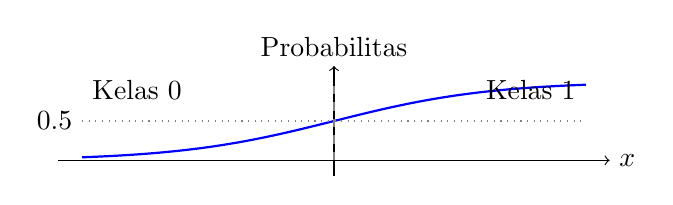
\begin{tikzpicture}[scale=1]
		% Axis
		\draw[->] (-3.5,0) -- (3.5,0) node[right] {$x$};
		\draw[->] (0,-0.2) -- (0,1.2) node[above] {Probabilitas};
		
		% Sigmoid curve
		\draw[thick, domain=-3.2:3.2, samples=100, smooth, variable=\x, blue]
		plot ({\x}, {1/(1 + exp(-\x))});
		
		% Dotted line at x=0
		\draw[dashed, gray] (0,0) -- (0,1);
		
		% Labels for class separation
		\node at (-2.5,0.9) {Kelas 0};
		\node at (2.5,0.9) {Kelas 1};
		
		% Threshold line
		\draw[dotted, gray] (-3.2,0.5) -- (3.2,0.5);
		\node[left] at (-3.2,0.5) {$0.5$};
		
	\end{tikzpicture}
	\caption{Logistic Regression – kurva S untuk memisahkan dua kelas.}
\end{figure}

\subsection*{3. Decision Tree}

\textbf{Decision Tree} meniru cara manusia mengambil keputusan berdasarkan logika “jika–maka” yang digambarkan dalam bentuk struktur pohon. Setiap cabang mewakili kondisi pada suatu fitur, dan setiap daun (leaf) merupakan prediksi akhir.  
Contoh: untuk mengevaluasi apakah seseorang layak mendapat pinjaman, decision tree dapat memeriksa atribut seperti penghasilan, usia, status pekerjaan, dan histori kredit.  
Keunggulan utamanya adalah transparansi — pengguna bisnis dapat memahami dan menelusuri alasan di balik prediksi model.

\begin{figure}[h]
	\centering
	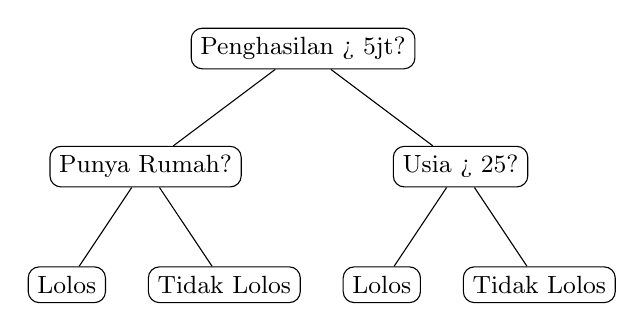
\begin{tikzpicture}[
		level 1/.style={sibling distance=40mm},
		level 2/.style={sibling distance=20mm},
		level distance=15mm,
		every node/.style={draw, rectangle, rounded corners, align=center, font=\small}
		]
		
		\node {Penghasilan > 5jt?}
		child {node {Punya Rumah?}
			child {node {Lolos}}
			child {node {Tidak Lolos}}
		}
		child {node {Usia > 25?}
			child {node {Lolos}}
			child {node {Tidak Lolos}}
		};
		
	\end{tikzpicture}
	\caption{Contoh struktur Decision Tree sederhana untuk evaluasi kelayakan pinjaman.}
\end{figure}

\subsection*{4. K-Nearest Neighbours (K-NN)}

\textbf{K-Nearest Neighbours (K-NN)} bekerja dengan membandingkan data baru dengan data historis yang paling mirip (berdekatan secara “jarak”).  
Model ini tidak membangun fungsi atau pohon, tapi menyimpan semua data historis dan membuat prediksi berdasarkan mayoritas “tetangga terdekat”.  
Contoh: jika ingin mengklasifikasikan tipe pelanggan baru, K-NN akan melihat siapa pelanggan lama yang mirip dari sisi profil dan perilaku, kemudian mengikuti kelompok mayoritas.

\begin{figure}[h]
	\centering
	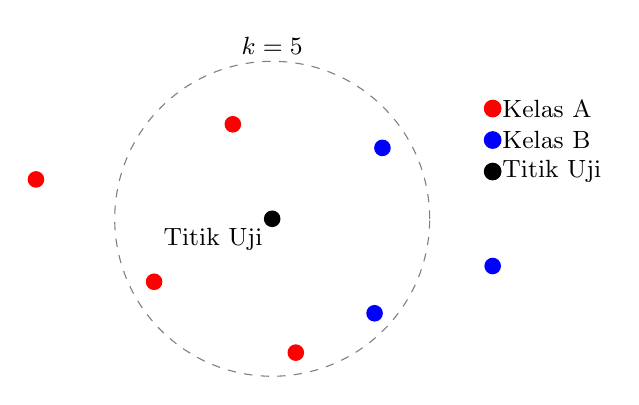
\begin{tikzpicture}[scale=1, every node/.style={font=\small}]
		
		% Titik uji (query point)
		\fill[black] (0,0) circle (3pt);
		\node[below left] at (0,0) {Titik Uji};
		
		% Lingkaran tetangga terdekat (misalnya radius k=5)
		\draw[gray, dashed] (0,0) circle (2);
		
		% Titik-titik kelas merah
		\fill[red] (-0.5, 1.2) circle (3pt);
		\fill[red] (-1.5, -0.8) circle (3pt);
		\fill[red] (0.3, -1.7) circle (3pt);
		
		% Titik-titik kelas biru
		\fill[blue] (1.4, 0.9) circle (3pt);
		\fill[blue] (1.3, -1.2) circle (3pt);
		
		% Titik luar radius (tidak dihitung)
		\fill[red] (-3, 0.5) circle (3pt);
		\fill[blue] (2.8, -0.6) circle (3pt);
		
		% Legenda
		\draw[red, fill=red] (2.8,1.4) circle (3pt);
		\node[right] at (2.8,1.4) {Kelas A};
		
		\draw[blue, fill=blue] (2.8,1.0) circle (3pt);
		\node[right] at (2.8,1.0) {Kelas B};
		
		\draw[black, fill=black] (2.8,0.6) circle (3pt);
		\node[right] at (2.8,0.6) {Titik Uji};
		
		% Label radius k
		\node at (0,2.2) {$k = 5$};
		
	\end{tikzpicture}
	\caption{K-NN – prediksi berdasarkan mayoritas kategori dari 5 tetangga terdekat.}
\end{figure}

\subsection*{Catatan Tambahan}

Pemilihan algoritma tergantung pada jenis data, tujuan prediksi, serta preferensi interpretabilitas.  
Dalam konteks bisnis, decision tree dan linear/logistic regression sering menjadi pilihan awal karena hasilnya mudah dipahami dan dikomunikasikan kepada manajemen \cite{provost2013data}.


\section{Tahapan Proyek Machine Learning dalam Big Data}

Proyek Machine Learning (ML), khususnya supervised learning, mengikuti alur sistematis yang memastikan model dibangun berdasarkan data yang relevan dan dapat digunakan secara efektif untuk mendukung keputusan bisnis. Dalam konteks Big Data, setiap tahap menghadapi tantangan tersendiri karena volume data yang besar, kecepatan pembaruan data, dan keragaman format sumbernya \cite{chen2012,wamba2017}.

Berikut adalah tahapan umum dalam proyek supervised learning dan bagaimana masing-masing terhubung dengan praktik Big Data for Business:

\subsection*{1. Mengumpulkan Data (Data Collection)}

Langkah awal adalah mengumpulkan data dari berbagai sumber: sistem transaksi, sensor IoT, media sosial, CRM, ERP, dan lainnya. Dalam konteks Big Data, tantangan utama adalah:
\begin{itemize}
	\item Volume data yang besar dan terus bertambah,
	\item Variasi format: terstruktur (CSV, database), semi-terstruktur (JSON, XML), dan tidak terstruktur (teks, gambar, audio),
	\item Sering kali data bersifat real-time atau streaming.
\end{itemize}

Pemanfaatan teknologi Big Data seperti Apache Kafka, NiFi, dan Hadoop HDFS umum digunakan dalam proses ini.

\subsection*{2. Membersihkan dan Menyiapkan Data (Data Preparation)}

Data yang dikumpulkan tidak selalu siap pakai. Proses ini melibatkan:
\begin{itemize}
	\item Menghapus duplikasi dan outlier,
	\item Menangani nilai yang hilang (missing values),
	\item Mengubah format dan skala data (normalisasi),
	\item Encoding variabel kategori menjadi angka,
	\item Memilih fitur (feature selection) yang relevan.
\end{itemize}

Pada tahap ini, kualitas data sangat menentukan kualitas model. Dalam konteks Big Data, pendekatan otomatis seperti pipeline data preparation sangat dibutuhkan untuk efisiensi dan skalabilitas \cite{rahm2000dataquality}.

\subsection*{3. Memilih Algoritma}

Bergantung pada tujuan bisnis dan jenis label:
\begin{itemize}
	\item Klasifikasi: Logistic Regression, Decision Tree, Random Forest, SVM.
	\item Regresi: Linear Regression, Gradient Boosting.
\end{itemize}

Faktor lain yang memengaruhi pilihan algoritma antara lain:
\begin{itemize}
	\item Ukuran dataset,
	\item Kebutuhan interpretabilitas,
	\item Waktu komputasi,
	\item Dukungan sistem operasional untuk model tersebut.
\end{itemize}

\subsection*{4. Melatih Model (Model Training)}

Model dilatih menggunakan data historis yang telah dipisahkan menjadi \texttt{training set}. Model belajar dari pola hubungan antara fitur dan label.  
Dalam skala Big Data, proses pelatihan sering membutuhkan pemrosesan paralel, distribusi data, dan optimalisasi beban kerja.

Tools seperti Apache Spark MLlib, TensorFlow, atau Orange (untuk pendekatan visual) umum digunakan.

\subsection*{5. Mengevaluasi Model (Model Evaluation)}

Model kemudian diuji pada \texttt{testing set} untuk mengevaluasi kemampuannya dalam memprediksi data yang belum pernah dilihat.  
Metrik evaluasi bergantung pada tipe prediksi:
\begin{itemize}
	\item \textbf{Klasifikasi:} akurasi, precision, recall, F1-score, ROC-AUC.
	\item \textbf{Regresi:} MAE (mean absolute error), RMSE (root mean squared error), R\textsuperscript{2} score.
\end{itemize}

Evaluasi dalam konteks bisnis juga mempertimbangkan \textit{nilai ekonomis} dari hasil model, bukan hanya performa statistik semata.

\subsection*{6. Menginterpretasikan Hasil untuk Pengambilan Keputusan}

Tahap akhir, tetapi paling kritikal dalam konteks bisnis. Hasil model harus:
\begin{itemize}
	\item Dipahami oleh pemangku kepentingan non-teknis,
	\item Diintegrasikan ke dalam proses bisnis (misalnya sistem rekomendasi, CRM, atau dashboard operasional),
	\item Disertai analisis risiko dan potensi bias algoritmik.
\end{itemize}

Keterlibatan pengguna bisnis dalam interpretasi hasil model sangat penting agar keputusan yang diambil berbasis data namun tetap mempertimbangkan konteks dan strategi organisasi \cite{provost2013data,davenport2018}.

\bigskip

\noindent
Seluruh tahapan ini sebaiknya dilakukan dalam pendekatan iteratif dan kolaboratif antara tim data dan pemangku kepentingan bisnis. Kerangka seperti CRISP-DM atau Data Value Chain dapat digunakan sebagai panduan metodologis.



\section{Praktik Hands-On dengan Orange}

\subsection{Langkah-langkah Menggunakan Orange}

Orange merupakan perangkat lunak open-source untuk analisis data dan pembelajaran mesin yang dirancang khusus bagi pengguna non-teknis. Dengan antarmuka visual berbasis \textit{drag-and-drop}, Orange memungkinkan mahasiswa untuk membangun alur analisis data secara intuitif tanpa memerlukan keterampilan pemrograman. Dalam praktik ini, mahasiswa akan memanfaatkan Orange untuk memvisualisasikan dan membangun model pohon keputusan berdasarkan dataset persetujuan pinjaman \texttt{loan.csv}.

Berikut adalah langkah-langkah praktis yang dapat diikuti:

\begin{enumerate}
	\item \textbf{Menginstal Orange:} 
	Kunjungi \url{https://orangedatamining.com}. Unduh dan instal aplikasi Orange. Aplikasi ini tersedia untuk Windows, macOS, dan Linux tanpa perlu konfigurasi tambahan.
	
	\item \textbf{Mempersiapkan Dataset:} 
	Gunakan dataset \texttt{data/loan.csv}\footnote{\url{https://u.pcloud.link/publink/show?code=kZnR3B5Z8TazEXoFXx7LJ4K87WksvXM0gu1X}} yang berisi data simulasi pengajuan pinjaman. Pastikan file disimpan dalam format \texttt{CSV} dan memiliki struktur kolom seperti: \texttt{employment\_status}, \texttt{income\_level}, \texttt{credit\_score}, \texttt{has\_collateral}, dan \texttt{loan\_approved}.
	
	\item \textbf{Membangun Workflow Analisis di Orange:}
	Buka Orange dan buat alur kerja (workflow) baru. Tambahkan dan hubungkan komponen-komponen berikut secara berurutan:
	\begin{itemize}
		\item \textbf{File:} Digunakan untuk memuat dataset \texttt{loan.csv}.
		\item \textbf{Data Table:} Menampilkan data dalam bentuk tabel dan memungkinkan eksplorasi awal.
		\item \textbf{Select Columns:} Untuk menentukan atribut input (fitur) dan variabel target.
		\item \textbf{Tree:} Komponen untuk membangun dan menampilkan model pohon keputusan.
	\end{itemize}
	
	\item \textbf{Menentukan Target dan Fitur:} 
	Pada komponen \texttt{Select Columns}, tetapkan \texttt{loan\_approved} sebagai variabel target. Atribut lainnya seperti \texttt{employment\_status}, \texttt{income\_level}, \texttt{credit\_score}, dan \texttt{has\_collateral} ditetapkan sebagai input features.
	
	\item \textbf{Menginterpretasikan Hasil:}
	Perhatikan fitur mana yang paling berkontribusi terhadap keputusan akhir. Jalur logika pada pohon membantu mengidentifikasi kombinasi atribut yang mendukung persetujuan pinjaman, serta mengilustrasikan bagaimana lembaga keuangan dapat membentuk strategi seleksi kredit yang lebih baik.
\end{enumerate}

Melalui praktik ini, mahasiswa tidak hanya mempelajari aspek teknis dari pohon keputusan, tetapi juga memahami bagaimana data historis dapat digunakan untuk menyusun kebijakan pinjaman yang berbasis data. Orange memberikan pengalaman langsung terhadap konsep \textit{self-service analytics}, di mana pengambil keputusan dapat melakukan eksplorasi data secara mandiri tanpa ketergantungan pada tim teknis \cite{demsar2013orange}. Konfigurasi alur kerja analisis ini di dalam Orange ditunjukkan pada Gambar~\ref{fig:pipeline-orange}.

\begin{figure}[h]
	\centering
	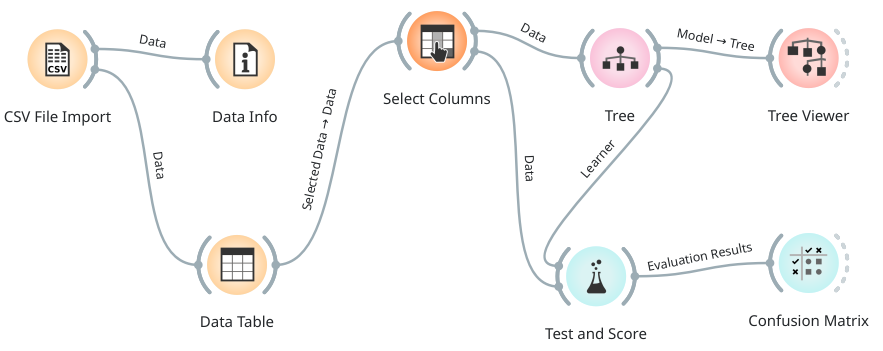
\includegraphics[width=\linewidth]{../figures/decision_tree_pipeline.png}
	\caption{Konfigurasi pipeline Orange untuk membangun decision tree dari dataset \texttt{loan.csv}}
	\label{fig:pipeline-orange}
\end{figure}




\subsection{Membangun Decision Tree dari Dataset Pinjaman}

Setelah dataset \texttt{loan.csv} dimuat dan atribut target (\texttt{loan\_approved}) ditentukan, langkah selanjutnya adalah membangun model pohon keputusan untuk memprediksi kemungkinan persetujuan pinjaman oleh lembaga keuangan. Decision tree dipilih karena model ini bersifat transparan, mudah dipahami, dan dapat divisualisasikan secara hierarkis, sehingga sangat cocok untuk kebutuhan analisis manajerial dalam dunia keuangan \cite{camm2020business}.

Di dalam Orange, pembangunan decision tree dilakukan melalui komponen \texttt{Tree}. Komponen ini secara otomatis menghasilkan model klasifikasi berdasarkan variabel input yang telah ditentukan. Prosesnya meliputi:

\begin{enumerate}
	\item \textbf{Pemilihan Atribut Pemisah (Splitting Criteria):} Orange secara default menggunakan \textit{Information Gain} atau \textit{Gini Index} untuk menentukan atribut terbaik di setiap node. Atribut ini menjadi dasar pemisahan data yang paling informatif terhadap variabel target.
	
	\item \textbf{Pembuatan Struktur Pohon:} Setelah atribut terbaik ditemukan, data dibagi ke dalam cabang-cabang berdasarkan nilai atribut tersebut. Proses ini berlanjut secara rekursif hingga pohon selesai terbentuk atau mencapai batasan tertentu, seperti kedalaman maksimum.
	
	\item \textbf{Pengendalian Overfitting:} Untuk menghindari kompleksitas model yang berlebihan, Orange menyediakan pengaturan seperti pembatasan kedalaman maksimum (\texttt{Max depth}), jumlah minimum data per simpul, dan metode pruning. Pengaturan ini dapat disesuaikan untuk menjaga keseimbangan antara akurasi dan interpretabilitas.
\end{enumerate}

Dalam praktik ini, mahasiswa disarankan untuk:

\begin{itemize}
	\item Membandingkan model pohon dengan kedalaman yang berbeda untuk memahami hubungan antara kompleksitas model dan kemudahan interpretasi.
	\item Mengamati simpul keputusan utama (root node) dan mendiskusikan alasan atribut tersebut dipilih sebagai pemisah awal.
	\item Mengevaluasi simpul daun (leaf nodes) untuk mengenali kombinasi karakteristik nasabah yang mengarah pada persetujuan (\texttt{Yes}) atau penolakan (\texttt{No}) pinjaman.
\end{itemize}

Sebagai contoh, model dapat menunjukkan bahwa nasabah dengan status pekerjaan \texttt{Employed}, tingkat pendapatan \texttt{Medium}, skor kredit \texttt{Good}, dan memiliki jaminan (\texttt{has\_collateral = True}) cenderung lebih mungkin mendapatkan persetujuan pinjaman. Pola semacam ini dapat dijadikan dasar untuk menyusun kebijakan pemberian kredit yang lebih efisien dan berbasis data.

Melalui eksplorasi visual di Orange, mahasiswa dapat memahami bagaimana pohon keputusan bekerja serta bagaimana pola-pola dalam data nasabah diterjemahkan menjadi logika bisnis yang dapat diterapkan secara nyata \cite{demsar2013orange}. 

\subsection{Visualisasi, Interpretasi Hasil, dan Insight Bisnis}

Salah satu keunggulan utama dari decision tree adalah kemampuannya untuk divisualisasikan dalam bentuk diagram pohon yang mudah dibaca. Dalam Orange, hasil pemodelan decision tree dapat ditampilkan secara interaktif melalui komponen \texttt{Tree Viewer}, yang memperlihatkan struktur node dan cabang berdasarkan pembagian data pada setiap atribut. Hal ini memudahkan manajer dan analis non-teknis untuk memahami logika di balik klasifikasi yang dihasilkan \cite{camm2020business}.

Setiap simpul dalam pohon menunjukkan kondisi yang digunakan untuk membagi data, seperti:
\begin{itemize}
	\item \texttt{credit\_score = Good}
	\item \texttt{has\_collateral = True}
	\item \texttt{income\_level = Medium}
\end{itemize}
dan setiap cabang menunjukkan kemungkinan hasil berdasarkan kondisi tersebut. Simpul daun (leaf node) akan berisi prediksi akhir (\texttt{Yes} atau \texttt{No}), jumlah observasi yang masuk ke simpul tersebut, serta persentase distribusi kelas berdasarkan data pelatihan.

Interpretasi dari hasil ini dapat membantu mahasiswa menjawab pertanyaan strategis, seperti:
\begin{itemize}
	\item Profil nasabah seperti apa yang paling mungkin disetujui pengajuan pinjamannya?
	\item Atribut mana yang paling menentukan keputusan persetujuan kredit?
	\item Bagaimana alur logika model dapat mendukung kebijakan pinjaman yang berbasis segmentasi risiko?
\end{itemize}

Sebagai contoh, hasil visualisasi dapat menunjukkan bahwa nasabah yang:
\begin{enumerate}
	\item memiliki skor kredit \texttt{Good},
	\item memiliki jaminan (\texttt{has\_collateral = True}), dan
	\item bekerja sebagai \texttt{Employed},
\end{enumerate}
memiliki probabilitas tinggi untuk mendapatkan persetujuan pinjaman. Struktur pohon keputusan yang dihasilkan dari dataset \texttt{loan.csv} ditampilkan pada Gambar~\ref{fig:loan-tree}.

\begin{figure}[h]
	\centering
	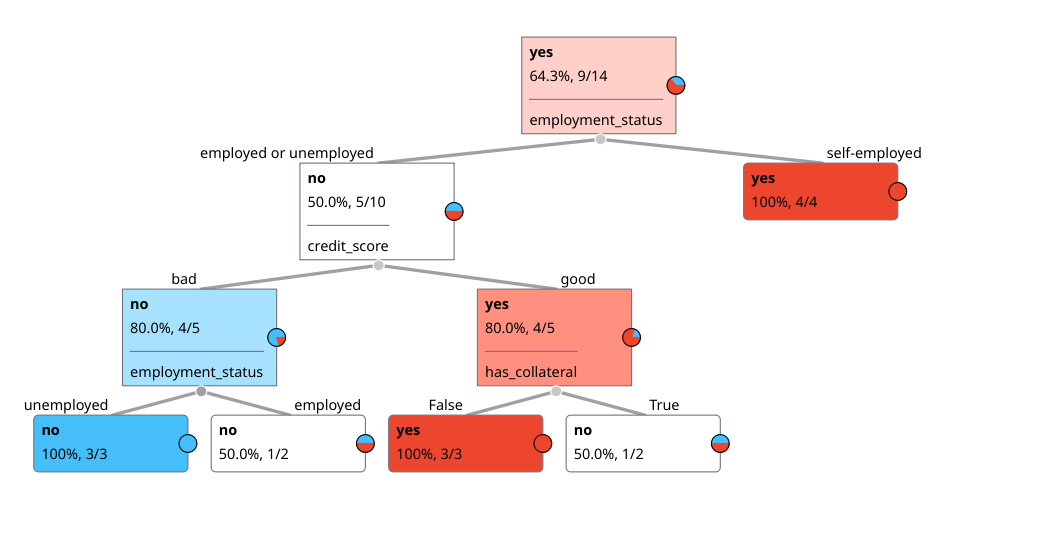
\includegraphics[width=\linewidth]{../figures/loan_tree.png}
	\caption{Visualisasi pohon keputusan hasil pemodelan dari dataset \texttt{loan.csv} di Orange}
	\label{fig:loan-tree}
\end{figure}

Insight dari model ini dapat dimanfaatkan oleh manajer risiko dan analis kredit untuk:
\begin{itemize}
	\item memprioritaskan aplikasi dari segmen berisiko rendah,
	\item menyusun kriteria kelayakan pinjaman yang lebih akurat, serta
	\item meningkatkan efisiensi dalam proses evaluasi kredit.
\end{itemize}

Visualisasi pohon keputusan juga memfasilitasi pendekatan \textit{what-if analysis}, di mana pengguna dapat menelusuri bagaimana perubahan pada atribut tertentu (misalnya, status pekerjaan atau keberadaan jaminan) dapat mengubah hasil prediksi. Ini menjadi sarana pembelajaran eksploratif yang sangat bermanfaat bagi mahasiswa manajemen yang sedang mempelajari konsep dasar analisis prediktif dan pengambilan keputusan berbasis data \cite{demsar2013orange}.

Dengan demikian, decision tree tidak hanya memberikan akurasi prediksi, tetapi juga mendukung penyusunan strategi bisnis yang lebih berbasis fakta, terukur, dan dapat dikomunikasikan secara lintas fungsi dalam organisasi.


\subsection{Eksplorasi Skema What-If dan Segmentasi Nasabah}

Salah satu keunggulan utama dari decision tree dalam konteks manajerial adalah kemampuannya untuk digunakan dalam eksplorasi skenario “what-if”. Pendekatan ini memungkinkan pengguna untuk mengevaluasi bagaimana perubahan nilai pada satu atau lebih atribut dapat memengaruhi hasil prediksi. Dalam Orange, mahasiswa dapat secara visual mengikuti jalur dalam pohon keputusan dan mengganti nilai atribut untuk melihat dampaknya terhadap keputusan akhir \cite{demsar2013orange}.

Sebagai contoh, jika seorang calon peminjam awalnya memiliki atribut:
\begin{itemize}
	\item \texttt{employment\_status = Unemployed},
	\item \texttt{credit\_score = Bad},
	\item \texttt{has\_collateral = False},
\end{itemize}
dan hasil prediksi menunjukkan \texttt{loan\_approved = No}, maka mahasiswa dapat mengganti nilai atribut menjadi:
\begin{itemize}
	\item \texttt{employment\_status = Employed},
	\item \texttt{credit\_score = Good},
	\item \texttt{has\_collateral = True},
\end{itemize}
untuk mengevaluasi apakah keputusan model berubah menjadi \texttt{loan\_approved = Yes}. Analisis seperti ini memberikan pemahaman mendalam tentang pengaruh relatif dari setiap atribut, serta dapat digunakan untuk menyusun kebijakan penyaringan kredit yang lebih adaptif.

Selain itu, decision tree juga secara alami menghasilkan \textbf{segmentasi nasabah} yang terstruktur. Setiap jalur dari root ke simpul daun dalam pohon merepresentasikan satu segmen dengan karakteristik unik. Misalnya, sebuah simpul daun mungkin berisi informasi seperti:

\begin{quote}
	“Nasabah dengan \texttt{employment\_status = Employed}, \texttt{income\_level = Medium}, \texttt{credit\_score = Good}, dan \texttt{has\_collateral = True} memiliki probabilitas tinggi untuk disetujui pinjamannya.”
\end{quote}

Segmentasi ini dapat dimanfaatkan oleh tim kredit atau manajemen risiko untuk:
\begin{enumerate}
	\item Menyusun kebijakan pinjaman yang lebih terarah berdasarkan profil peminjam yang berpotensi disetujui.
	\item Menyesuaikan persyaratan kredit dan skema bunga sesuai dengan karakteristik segmen tertentu.
	\item Melakukan prioritisasi pemrosesan aplikasi berdasarkan risiko dan potensi pengembalian.
\end{enumerate}

Pendekatan ini mendukung konsep \textit{data-driven segmentation}, di mana pengelompokan nasabah tidak hanya didasarkan pada intuisi, tetapi pada bukti empiris yang terstruktur dari hasil analitik. Dengan demikian, decision tree tidak hanya bertindak sebagai alat prediksi, tetapi juga sebagai alat eksplorasi strategi dan penyusunan kebijakan bisnis yang lebih presisi dan efektif \cite{camm2020business}.

Melalui eksplorasi skenario dan segmentasi ini, mahasiswa diharapkan mampu mengembangkan wawasan kritis dalam menyusun kebijakan keuangan atau layanan pelanggan yang responsif terhadap karakteristik dan perilaku peminjam yang berbeda-beda.



\section{Evaluasi Model dan Ukuran Kinerja}

Evaluasi model merupakan tahap krusial dalam supervised learning karena membantu menentukan apakah model yang dibangun mampu memberikan prediksi yang akurat dan relevan secara bisnis. Dalam konteks prediksi persetujuan pinjaman seperti pada praktik dengan Orange, evaluasi ini sangat penting untuk memastikan bahwa keputusan yang diambil berdasarkan model akan memberikan dampak positif terhadap efektivitas strategi kredit.

Orange menyediakan berbagai metrik evaluasi melalui komponen \texttt{Test \& Score}, yang dapat dihubungkan langsung ke model decision tree dan dataset. Komponen ini menghitung ukuran-ukuran kinerja utama seperti \textbf{accuracy}, \textbf{precision}, \textbf{recall}, dan \textbf{F1-score}, serta menyajikan ringkasan hasil dalam format tabel sederhana yang mudah dipahami. Berikut adalah penjelasan dari masing-masing metrik dan relevansinya dalam konteks bisnis:

\subsection*{1. Akurasi (Accuracy)}

Akurasi menunjukkan proporsi keseluruhan prediksi yang benar dibandingkan dengan total data. Misalnya, jika model memproses 100 data pengajuan pinjaman dan menghasilkan 85 prediksi yang sesuai dengan kenyataan, maka akurasinya adalah 85\%.

\textbf{Kelebihan:} Mudah dihitung dan dipahami.  
\textbf{Kekurangan:} Bisa menyesatkan jika distribusi kelas tidak seimbang, misalnya jika sebagian besar aplikasi pinjaman memang disetujui.

\subsection*{2. Precision}

Precision mengukur ketepatan model dalam memprediksi persetujuan pinjaman. Ini menunjukkan berapa banyak dari seluruh prediksi \texttt{Yes} (disetujui) yang memang benar-benar disetujui dalam kenyataannya.

\[
\text{Precision} = \frac{\text{True Positives}}{\text{True Positives + False Positives}}
\]

\textbf{Contoh:} Jika model memprediksi 40 pengajuan akan disetujui, tetapi hanya 30 yang benar-benar disetujui, maka precision = 75\%.

\textbf{Konteks bisnis:} Precision tinggi berarti lembaga keuangan tidak terlalu banyak menyetujui pinjaman untuk peminjam yang sebenarnya berisiko.

\subsection*{3. Recall (Sensitivity)}

Recall menunjukkan seberapa baik model dalam menemukan semua kasus persetujuan pinjaman yang seharusnya disetujui. Ini mengukur kemampuan model menangkap seluruh data positif yang benar.

\[
\text{Recall} = \frac{\text{True Positives}}{\text{True Positives + False Negatives}}
\]

\textbf{Contoh:} Jika ada 50 pengajuan yang seharusnya disetujui, dan model hanya berhasil menangkap 30, maka recall = 60\%.

\textbf{Konteks bisnis:} Recall tinggi penting untuk memastikan lembaga tidak kehilangan peluang dari nasabah yang sebenarnya layak menerima pinjaman.

\subsection*{4. F1-Score}

F1-score adalah ukuran keseimbangan antara precision dan recall, menggunakan rata-rata harmonis dari keduanya. Metode ini digunakan ketika kedua aspek—ketepatan dan kelengkapan—sama pentingnya.

\[
\text{F1-Score} = 2 \times \frac{\text{Precision} \times \text{Recall}}{\text{Precision} + \text{Recall}}
\]

\textbf{Konteks bisnis:} F1-score menjadi pilihan utama ketika lembaga ingin menghindari terlalu banyak kesalahan prediksi dalam dua arah: menyetujui pinjaman yang seharusnya ditolak, dan menolak pinjaman yang seharusnya disetujui.

\subsection*{Pemilihan Metrik Berdasarkan Tujuan Analisis}

Tidak ada satu metrik yang selalu paling cocok dalam semua situasi. Pemilihan metrik harus disesuaikan dengan strategi dan konteks bisnis:

\begin{itemize}
	\item Jika \textbf{risiko kredit macet sangat tinggi}, maka precision lebih diutamakan untuk menghindari persetujuan kepada peminjam yang tidak layak.
	\item Jika \textbf{lembaga ingin meningkatkan inklusi keuangan}, recall menjadi penting agar tidak banyak peminjam yang layak justru ditolak.
	\item Jika ingin \textbf{menyeimbangkan kedua risiko tersebut}, maka F1-score digunakan untuk memberikan gambaran performa yang lebih proporsional.
\end{itemize}

Melalui pendekatan ini, mahasiswa tidak hanya memahami angka-angka dari hasil evaluasi model, tetapi juga bagaimana mengaitkan metrik tersebut dengan dampaknya terhadap strategi dan kebijakan bisnis. Orange menyediakan platform evaluasi yang ramah pengguna sehingga proses penilaian performa model dapat dilakukan secara visual, iteratif, dan intuitif tanpa memerlukan pemrograman.

\section{Evaluasi Praktik Hands-On}

\begin{figure}[h]
	\centering
	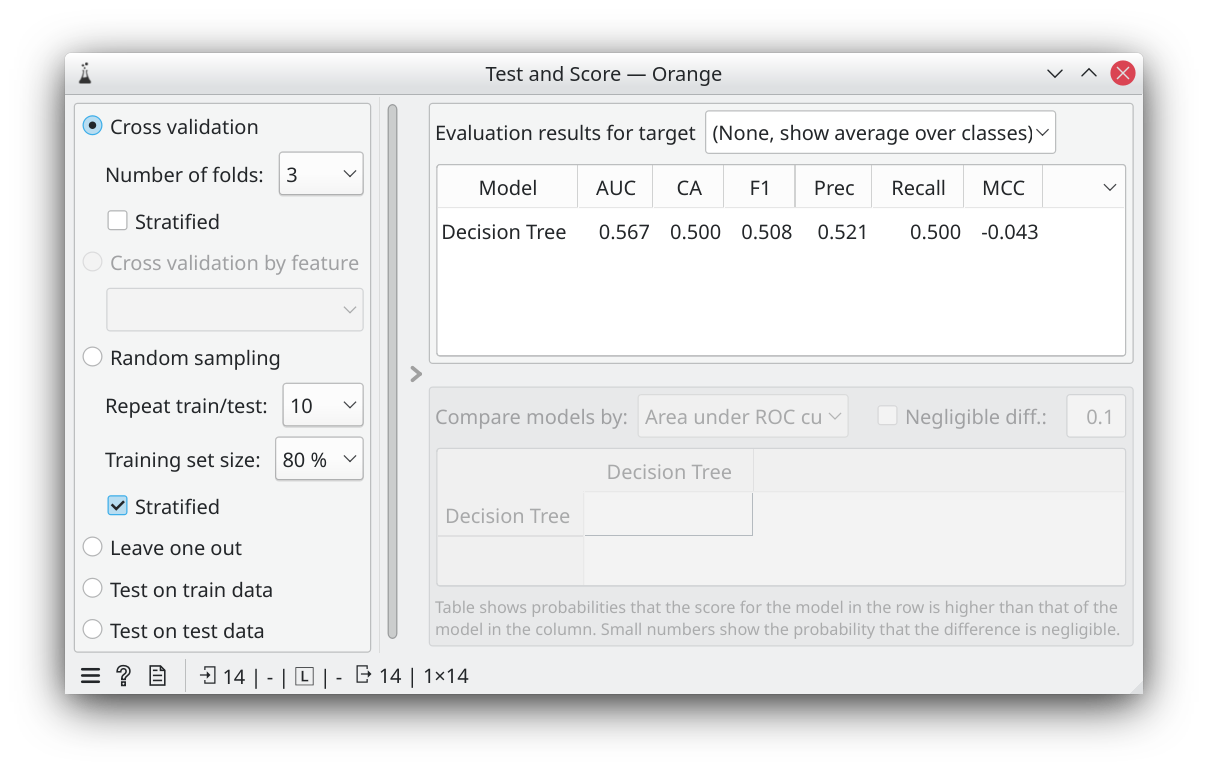
\includegraphics[width=0.9\linewidth]{../figures/decision_tree_results.png}
	\caption{Hasil evaluasi model Decision Tree pada Orange.}
\end{figure}

Evaluasi dilakukan menggunakan perangkat lunak \textit{Orange} untuk menilai kinerja model \textit{Decision Tree} terhadap dataset klasifikasi. Evaluasi dilakukan melalui widget \textit{Test and Score} dengan konfigurasi sebagai berikut:

\begin{itemize}
	\item \textbf{Metode evaluasi:} Cross Validation
	\item \textbf{Jumlah fold:} 3 (3-Fold Cross Validation)
	\item \textbf{Stratified:} Dicentang (Stratified)
	\item \textbf{Model:} Decision Tree
\end{itemize}

\textbf{Cross Validation} adalah teknik evaluasi di mana dataset dibagi menjadi beberapa bagian yang disebut \textit{fold}. Dalam konfigurasi 3-fold, data dibagi menjadi tiga bagian yang seimbang. Setiap fold secara bergiliran digunakan sebagai data uji, sementara dua fold lainnya digunakan sebagai data latih. Proses ini dilakukan sebanyak tiga kali, dan hasil evaluasi dirata-ratakan.

\textbf{Stratified Cross Validation} berarti bahwa distribusi kelas (label) dalam setiap fold dibuat serupa dengan distribusi asli pada dataset. Ini penting untuk menghindari ketimpangan kelas di salah satu fold, terutama pada data klasifikasi dengan distribusi tidak seimbang.

\subsection*{Hasil Evaluasi}

Berikut adalah nilai-nilai metrik yang dihasilkan dari proses evaluasi model Decision Tree:

\begin{center}
	\begin{tabular}{|l|c|}
		\hline
		\textbf{Metrik} & \textbf{Nilai} \\
		\hline
		AUC (Area Under Curve) & 0.567 \\
		CA (Classification Accuracy) & 0.500 \\
		F1 Score & 0.508 \\
		Precision & 0.521 \\
		Recall & 0.500 \\
		MCC (Matthews Correlation Coefficient) & -0.043 \\
		\hline
	\end{tabular}
\end{center}

\subsection*{Interpretasi Hasil Evaluasi}

\begin{itemize}
	\item \textbf{AUC (Area Under Curve)} mengukur kemampuan model untuk membedakan antar kelas. Nilai 0.567 sedikit di atas nilai acak (0.5), artinya model memiliki kemampuan terbatas untuk membedakan kelas target.
	
	\item \textbf{Classification Accuracy (CA)} sebesar 0.500 menunjukkan bahwa hanya 50\% dari seluruh prediksi model yang sesuai dengan label sebenarnya. Ini berarti model hanya benar separuh waktu.
	
	\item \textbf{F1 Score} adalah rata-rata harmonis antara precision dan recall. Nilai 0.508 menunjukkan bahwa performa model cukup seimbang antara kemampuan mengenali kelas positif dan ketepatan dalam prediksi, tetapi masih berada di level sedang.
	
	\item \textbf{Precision} sebesar 0.521 berarti dari semua prediksi positif yang diberikan oleh model, sekitar 52.1\% di antaranya benar-benar positif.
	
	\item \textbf{Recall} sebesar 0.500 berarti bahwa model berhasil mengenali 50\% dari seluruh data yang seharusnya berlabel positif.
	
	\item \textbf{Matthews Correlation Coefficient (MCC)} sebesar -0.043 menunjukkan hampir tidak ada korelasi antara hasil prediksi model dan label sebenarnya. Nilai mendekati nol mengindikasikan bahwa model belum menunjukkan performa klasifikasi yang baik.
\end{itemize}

\subsection*{Kesimpulan Sementara}

Meskipun hasil evaluasi lebih baik dibandingkan sebelumnya, performa model Decision Tree masih tergolong rendah. AUC yang sedikit di atas 0.5 menunjukkan bahwa model belum optimal dalam membedakan antar kelas. Kemungkinan penyebabnya adalah:

\begin{enumerate}
	\item \textbf{Kompleksitas data yang tinggi} atau pola antar fitur yang tidak cukup kuat untuk dipelajari oleh model Decision Tree.
	\item \textbf{Ukuran dataset yang terbatas} menyebabkan model belum mampu generalisasi dengan baik.
	\item \textbf{Distribusi fitur yang kurang informatif} terhadap target variabel.
\end{enumerate}


\section{Analisis Confusion Matrix}

\begin{figure}[h]
	\centering
	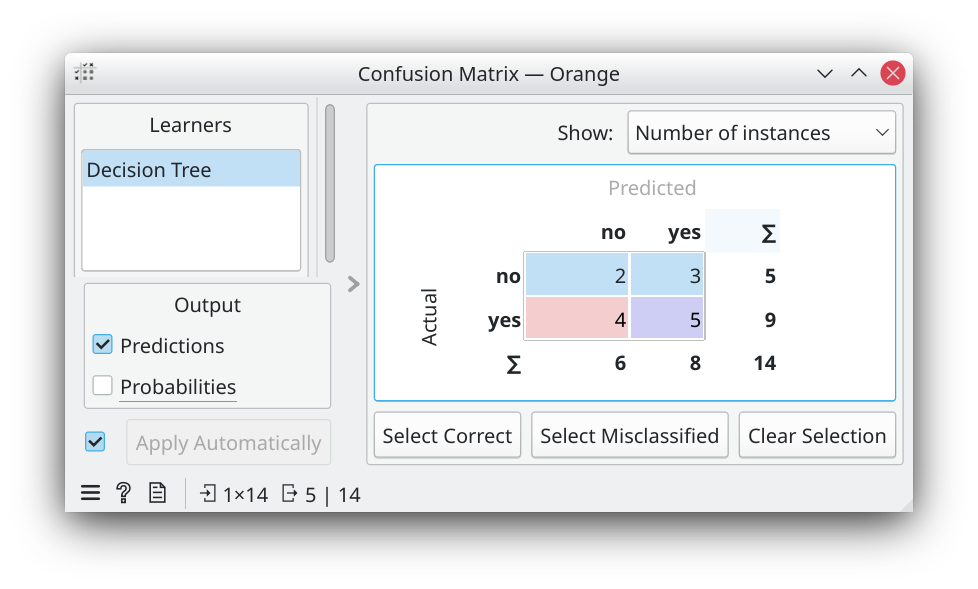
\includegraphics[width=0.7\linewidth]{../figures/decision_tree_confusion_matrix.png}
	\caption{Confusion Matrix untuk model Decision Tree pada Orange.}
\end{figure}

Confusion matrix digunakan untuk melihat secara detail performa klasifikasi berdasarkan jumlah prediksi yang benar dan salah pada masing-masing kelas. Gambar di atas menunjukkan hasil confusion matrix dari model \textit{Decision Tree} dengan dua kelas: \texttt{no} dan \texttt{yes}. 

Setiap sel dalam matriks menunjukkan jumlah instance yang diklasifikasikan pada masing-masing kombinasi kelas aktual dan kelas prediksi. Baris menyatakan label aktual, sedangkan kolom menyatakan prediksi model.

\subsection*{Isi Matriks}

\begin{center}
	\begin{tabular}{|c|c|c|c|}
		\hline
		& \textbf{Predicted: no} & \textbf{Predicted: yes} & \textbf{Total (Aktual)} \\
		\hline
		\textbf{Actual: no} & 2 (True Negative) & 3 (False Positive) & 5 \\
		\textbf{Actual: yes} & 4 (False Negative) & 5 (True Positive) & 9 \\
		\hline
		\textbf{Total (Prediksi)} & 6 & 8 & 14 \\
		\hline
	\end{tabular}
\end{center}

\subsection*{Interpretasi}

\begin{itemize}
	\item \textbf{True Positive (TP):} 5 — Kasus \texttt{yes} yang diprediksi benar sebagai \texttt{yes}.
	\item \textbf{True Negative (TN):} 2 — Kasus \texttt{no} yang diprediksi benar sebagai \texttt{no}.
	\item \textbf{False Positive (FP):} 3 — Kasus \texttt{no} yang salah diprediksi sebagai \texttt{yes}.
	\item \textbf{False Negative (FN):} 4 — Kasus \texttt{yes} yang salah diprediksi sebagai \texttt{no}.
\end{itemize}

\subsection*{Perhitungan Metrik Berdasarkan Confusion Matrix}

Dari nilai-nilai tersebut dapat dihitung ulang beberapa metrik dasar untuk validasi:

\begin{itemize}
	\item \textbf{Accuracy} = \( \frac{TP + TN}{TP + TN + FP + FN} = \frac{5 + 2}{14} = 0.500 \)
	\item \textbf{Precision} = \( \frac{TP}{TP + FP} = \frac{5}{5 + 3} = 0.625 \)
	\item \textbf{Recall} = \( \frac{TP}{TP + FN} = \frac{5}{5 + 4} = 0.556 \)
	\item \textbf{F1 Score} = \( 2 \times \frac{Precision \times Recall}{Precision + Recall} \approx 0.588 \)
\end{itemize}

Perlu dicatat bahwa nilai-nilai metrik dari confusion matrix ini dapat sedikit berbeda dari rata-rata yang ditampilkan pada hasil \textit{Test and Score}, karena confusion matrix biasanya dihitung dari agregasi keseluruhan prediksi (bukan rata-rata per fold).

\subsection*{Kesimpulan}

Model Decision Tree masih menunjukkan performa yang moderat. Dari confusion matrix terlihat bahwa model lebih sering salah dalam memprediksi kelas \texttt{yes} sebagai \texttt{no} (FN = 4), dan juga melakukan sejumlah kesalahan dalam memprediksi \texttt{no} sebagai \texttt{yes} (FP = 3). Untuk meningkatkan akurasi, disarankan eksplorasi model lain, tuning parameter, serta pemilihan fitur yang lebih relevan.


\section{Latihan Mandiri: Karakterisasi Churn Pelanggan dengan Decision Tree}

Gunakan dataset \textit{Telco Customer Churn} dari Kaggle untuk membangun model prediksi menggunakan decision tree di Orange. Dataset ini berisi data pelanggan layanan telekomunikasi dan status churn mereka (\texttt{Churn = Yes/No}).

\subsection*{Langkah Praktik}

\begin{enumerate}
	\item Kunjungi \url{https://www.kaggle.com/datasets/blastchar/telco-customer-churn}, kemudian unduh dataset.
	\item Buka Orange dan buat alur kerja (\textit{workflow}) dengan komponen. 
	\begin{itemize}
		\item \texttt{File} – untuk memuat \texttt{Telco-Customer-Churn.csv}
		\item \texttt{Select Columns} – atur \texttt{Churn} sebagai target
		\item \texttt{Data Table} – untuk melihat isi data
		\item \texttt{Tree} – untuk membangun model decision tree
	\end{itemize}
	\item Jalankan model dan amati atribut yang paling memengaruhi churn.
	\item Tampilkan hasil pohon dan simpulkan hasil analisis.
\end{enumerate}

\subsection*{Output yang Diharapkan}

\begin{itemize}
	\item Visual pohon keputusan dari Orange.
	\item Ringkasan interpretasi simpul utama.
	\item Rekomendasi singkat berdasarkan hasil model.
	\item Hasil Evaluasi
\end{itemize}


\section{Rangkuman}

Machine Learning (ML), khususnya pendekatan supervised learning, merupakan tahap lanjutan dalam strategi Big Data yang berfokus pada penciptaan nilai melalui analitik prediktif dan preskriptif. Setelah data dikumpulkan, disimpan, dan diproses, ML memungkinkan organisasi tidak hanya memahami apa yang terjadi di masa lalu (descriptive analytics), tetapi juga memprediksi apa yang akan terjadi dan merekomendasikan tindakan terbaik yang dapat diambil (prescriptive analytics) \cite{provost2013data}. Dalam konteks bisnis, ML menjadi enabler utama bagi pengambilan keputusan berbasis data, yang lebih cepat, akurat, dan relevan terhadap kondisi pasar yang dinamis.

Ke depan, organisasi dapat mengeksplorasi pendekatan lanjutan seperti AutoML (automated machine learning) untuk menyederhanakan proses pemodelan, serta mengintegrasikan hasil ML ke dalam dashboard interaktif yang mudah diinterpretasi oleh manajemen. Visualisasi hasil prediksi, pelacakan kinerja model, dan pembaruan model berbasis data baru merupakan aspek penting dalam integrasi ML dengan sistem pengambilan keputusan sehari-hari. Dengan membangun budaya data-driven dan tata kelola data yang kuat, Machine Learning dapat dioptimalkan sebagai aset strategis dalam keseluruhan arsitektur Big Data for Business.
